\section{LLR Quality and Recalibration}
\label{sec:llr}

A code-review pass over the finished system asked a simple question:
are the demodulator's LLRs actually calibrated --- does $|L|$ mean
what it claims?  Measuring them against ground truth
(\texttt{experiments/llr\_calibration.py}) found the single largest
untapped gain in the system.

\subsection{The Miscalibration Is Shape, Not Temperature}

Two terms are used throughout this section and deserve definition.
\emph{Temperature scaling} is the standard one-parameter recalibration
family
\begin{equation}
    L' \;=\; \alpha \cdot L, \qquad \alpha > 0,
\end{equation}
one global gain applied uniformly to every LLR.  The name comes from
machine-learning calibration~\cite{guo2017calibration}, where a
network's logits are divided by a scalar ``temperature'' $T$ before
the softmax ($\alpha \equiv 1/T$) --- itself borrowed from the
Boltzmann distribution, in which temperature controls how sharply
probability concentrates on the most likely outcome: $\alpha < 1$
softens overconfident beliefs, $\alpha > 1$ sharpens underconfident
ones.  It is the natural first candidate here because it preserves
signs and ordering, costs one multiply, and can be fitted blind on a
per-frame basis: a correctly calibrated Gaussian LLR ensemble
satisfies the consistency condition
$\operatorname{Var}[\ell] = 2\,\mathbb{E}[\ell]$ (for
$\ell = L \cdot \tilde{x}$, the LLR signed by the true bit), so the
moment estimator $\alpha = 2\,\mathbb{E}[\ell]/\operatorname{Var}[\ell]$
recovers the gain that restores consistency.  By contrast,
\emph{shape} refers to any monotone but non-linear correction
$L' = f(|L|) \cdot \operatorname{sgn} L$ --- one that can treat weak
and strong LLRs differently.  The finding of this section is that the
front end's miscalibration is of the second kind, so the first kind
cannot repair it.

The raw LLRs ($4\cdot\mathrm{Re}\cdot E_s/N_0$ per carrier, clipped to
$\pm 20$) are \emph{shape}-miscalibrated: bits with $|L|<2$ err 11\,\%
empirically versus the 39\,\% their value implies --- the
decision-directed noise estimation and per-carrier weighting
over-spread confidence downward --- while the clipped top of the scale
overstates.  A single temperature cannot fix this: the moment fit is
dragged by the clipped mass, and the fitted $\alpha<1$ while the weak
LLRs are empirically \emph{under}confident, a contradiction only a
shape correction resolves.  Figure~\ref{fig:llr_shape} shows the
measured shape.  In the left panel, the measured error rate starts
\emph{below} the ideal curve $P(\mathrm{err}) = 1/(1+e^{|L|})$ (weak
LLRs are better than they claim) and crosses it around $|L| \approx 5$,
after which errors run orders of magnitude \emph{above} the claim ---
and beyond $|L| \approx 9$ the measured reliability actually
\emph{decreases} as the claimed confidence rises, all the way into the
clipped mass at $|L| \approx 19$.
The right panel replots the same data as empirical log-odds versus
nominal $|L|$: a calibrated front end would sit on the identity line,
but the measured curve rises above it at small $|L|$ (wanting
$\alpha > 1$) and falls far below at large $|L|$ (dragging any global
fit to $\alpha < 1$ --- here $\alpha = 0.67$).  No straight line
through the origin can be on the correct side of both regions
simultaneously; the red curve itself, applied as a lookup, is the
monotone reliability map of the next subsection.  Note where the
measured curve peaks: $\approx 7.5$ empirical log-odds at
$|L| \approx 9$ --- the deployed map's cap of $7.4$ is that peak,
re-measured independently.  This is also the
figure that explains the LDPC result of Section~\ref{sec:coding}:
exact sum--product consumes these numbers as \emph{absolute}
probabilities and pays for every lie, while min-sum and Viterbi only
compare them.

\begin{figure}[H]
    \centering
    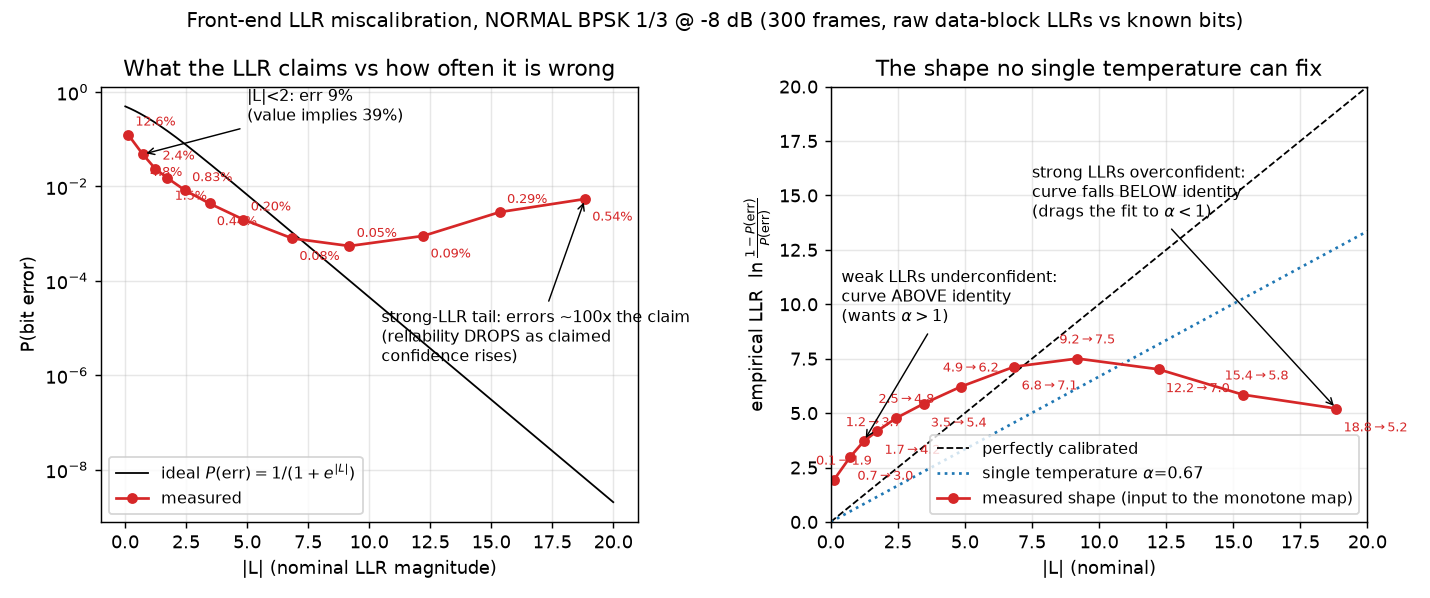
\includegraphics[width=\textwidth]{images/llr_shape.png}
    \caption{The measured LLR miscalibration shape (NORMAL BPSK 1/3
             at $-8$\,dB, 300 frames, raw data-block LLRs against
             known transmitted bits; reproduce with
             \texttt{experiments/llr\_shape.py}, bin table and
             parameters in \texttt{results/llr\_shape.json}).
             Left: claimed versus actual reliability, each bin
             annotated with its measured error rate.  Right: the same
             data as empirical log-odds, each point annotated with its
             mapping (nominal $\rightarrow$ empirical) --- above the
             identity line at small $|L|$, below it at large $|L|$, so
             no single temperature $\alpha$ can correct both ends.}
    \label{fig:llr_shape}
\end{figure}

\subsubsection{Measurement Procedure}
\label{sec:llr_procedure}

The data behind Figure~\ref{fig:llr_shape} (and behind the deployed
map of the next subsection) is produced by a self-labeling protocol
--- the transmitter's bit pipeline is deterministic, so every raw LLR
can be paired with the coded bit it was supposed to carry:

\begin{enumerate}
    \item \textbf{Stimulus.}  300 NORMAL-mode frames, BPSK rate 1/3,
          27-byte random payloads; each passes the channel simulator
          with a random start offset (300--1200 samples), a random
          CFO drawn uniformly from $\pm 60$\,Hz, and AWGN at the
          target SNR ($-8$\,dB here, 6\,kHz convention).  Collection
          runs as parallel 30-frame chunks with per-chunk seeds, so
          the run is reproducible and its result is recorded in
          \texttt{results/llr\_shape.json}.
    \item \textbf{Reception.}  Each frame goes through the
          \emph{production} receive chain --- preamble detection,
          CFO correction, tile accumulation, channel estimation, MMSE,
          LLR formation with the $\pm 20$ clip
          (Section~\ref{sec:llr_math}) --- and the raw data-block
          LLRs are captured \emph{before} any decoding or
          recalibration.  Frames that fail preamble detection are
          skipped; no selection is made on CRC, so decoding failures
          do not bias the sample.
    \item \textbf{Ground truth.}  The known payload is run through
          the TX bit pipeline (FEC encode $\to$ pad $\to$ interleave
          $\to$ scramble), giving the transmitted coded bit for every
          LLR position.  With $\tilde{x} = \pm 1$ ($+1 \Leftrightarrow$
          bit 1, the sign convention), each sample is reduced to the
          signed product $\ell = L \cdot \tilde{x}$: $\ell < 0$ means
          the LLR votes for the wrong bit, and $|\ell| = |L|$ is its
          claimed confidence.
    \item \textbf{Binning.}  Pooled samples are binned by $|\ell|$
          (edges $0, 0.5, 1, 1.5, 2, 3, 4, 6, 8, 11, 14, 17, 20$);
          bins with fewer than 80 samples are dropped.  Per bin, the
          empirical error rate is
          $\hat{p} = \operatorname{mean}(\ell < 0)$, clamped to
          $[\,0.5/N,\; 1 - 0.5/N\,]$ (a half-count continuity
          correction that keeps the log-odds finite when a bin has no
          errors), and the bin's abscissa is its mean $|\ell|$.
    \item \textbf{Derived quantities.}  The empirical log-odds
          $\hat{L} = \ln\bigl((1-\hat{p})/\hat{p}\bigr)$ give the
          right panel; the reference curve is
          $P(\mathrm{err}) = 1/(1+e^{|L|})$.  The single-temperature
          baseline is the moment fit
          \begin{equation}
              \alpha \;=\; \frac{2\,\mathbb{E}[\ell]}
                                {\operatorname{Var}[\ell]},
          \end{equation}
          the consistency condition of a well-calibrated Gaussian LLR
          ($\operatorname{Var} = 2\,\mathbb{E}$ under the standard
          approximation $L \sim \mathcal{N}(\pm\sigma^2/2, \sigma^2)$)
          --- the same estimator the runtime header-based temperature
          fit uses, which is exactly why the figure's $\alpha = 0.67$
          is representative of what deployment would apply.
\end{enumerate}

The harness is \texttt{experiments/llr\_calibration.py} (collection
and console reliability tables) and \texttt{experiments/llr\_shape.py}
(the figure and its JSON record); re-running either regenerates all
numbers from scratch.

\subsection{The Monotone Reliability Map}

The correction is a measured monotone map: each $|L|$ bin is replaced
by the log-odds of its empirical error rate (10 interior bin edges,
saturating at the data-justified maximum of $\approx$7.4).  Capping
LLRs at what the data supports also defuses confidently-wrong bits
from BSC flips and fades.  Measured at the sensitivity edge (NORMAL
BPSK 1/3, 40 trials/point):

\begin{table}[H]
    \centering
    \caption{Decodes out of 40 with and without recalibration.}
    \label{tab:recal}
    \small
    \begin{tabular}{@{}lrr@{}}
    \toprule
    \textbf{SNR} & \textbf{Raw LLRs} & \textbf{Recalibrated} \\
    \midrule
    $-8$\,dB & 33/40 & 38/40 \\
    $-9$\,dB & 6/40  & \textbf{29/40} \\
    \bottomrule
    \end{tabular}
\end{table}

This is $\approx$\textbf{1.5--2\,dB of sensitivity} for the existing
convolutional chain (Viterbi decoding is scale-invariant but not
shape-invariant), and it is what finally lets LDPC sum-product
decoding work on this front end (9/40 $\rightarrow$ 24/40 at
$-9$\,dB).  The accumulation-limited ROBUST/EXTREME rungs are
unaffected \emph{at their operating points} (re-measured at 300
frames/point in Section~\ref{sec:coding}: the map's gain at EXTREME
decays to zero by $-18$\,dB, though $\approx$0.5\,dB survives at the
deep edge below the rung), and 16-QAM \emph{regresses} under the
BPSK-trained map at the ladder rates (re-measured at 300 frames/point
in Section~\ref{sec:coding}: $-0.5$\,dB at rate 2/3, though at rate
1/3 the map actually helps --- the regression is rate-dependent), so
the map is gated to modulations with $\mu \le 2$ bits/symbol.

\subsection{Why the Map Helps Viterbi (and Temperature Cannot)}
\label{sec:viterbi_recal}

It is worth being precise about \emph{which} part of the calibration
each decoder consumes, because the two decoder families fail in
opposite ways:

\begin{itemize}
    \item \textbf{Temperature is provably useless for Viterbi.}  The
          path metric $\mathrm{PM} = \sum_e \beta_e$ is linear in the
          LLRs (Section~\ref{sec:coding}), so scaling every LLR by any
          $\alpha > 0$ scales every competing path metric by the same
          $\alpha$ --- the arg-max, and therefore every decoded bit,
          is unchanged.  Figure~\ref{fig:viterbi_recal} (left) shows
          this empirically: the temperature-only curve overlays the
          raw curve \emph{exactly}, frame for frame, at every SNR.
          Exact sum--product LDPC is the opposite case: its $\tanh$
          nonlinearity consumes absolute LLR values, so the scale
          error alone costs it dB.
    \item \textbf{Shape is what Viterbi actually consumes.}  The
          decoder compares \emph{sums} of LLRs along competing paths,
          so the decisive quantity is the relative weight of one
          strong bit against several weak ones.  The measured shape
          (Figure~\ref{fig:llr_shape}) breaks exactly that ratio: a
          raw $|L|=9$ bit claims to outweigh four $|L|=2$ bits, but
          its empirical log-odds are $\approx 6$ while each weak bit
          is really worth $\approx 4$.  Two failure modes follow.  A
          single confidently-wrong strong bit (fade, impulse) can
          outvote several correct weak bits along a path --- the
          map's cap at the data-justified $\approx 7.4$ defuses this.
          And underweighted weak bits waste real information --- the
          map restores their influence in the path sums.
    \item \textbf{HARQ combining needs calibrated addends.}  Chase
          combining adds the LLR streams of two receptions; if the
          two frames sit on different miscalibrated scales (different
          SNR, different noise-estimate transients), the sum weights
          the frames wrongly.  Mapping both to honest log-odds first
          makes addition the theoretically correct combining rule.
    \item \textbf{Puncturing is calibration-neutral.}  Depuncture
          zeros mean ``no opinion,'' and any odd monotone map keeps
          $0$ at $0$, so the inserted positions are unaffected by
          construction.
\end{itemize}

Figure~\ref{fig:viterbi_recal} makes the asymmetry measurable in one
sweep (300 frames per point): the same raw LLRs from each received
frame are decoded three ways.  Temperature-only reproduces the raw
decisions bit-exactly at every point --- 2\,700 frames without a
single divergence; the generating script asserts this equality, so
scale invariance is enforced, not eyeballed.  The monotone map shifts
the decode waterfall by $\approx$1.5\,dB: at $-9$\,dB, 63/300 raw
versus 216/300 mapped; at $-9.5$\,dB, 15/300 versus 165/300 ---
consistent with Table~\ref{tab:recal}.

\begin{figure}[H]
    \centering
    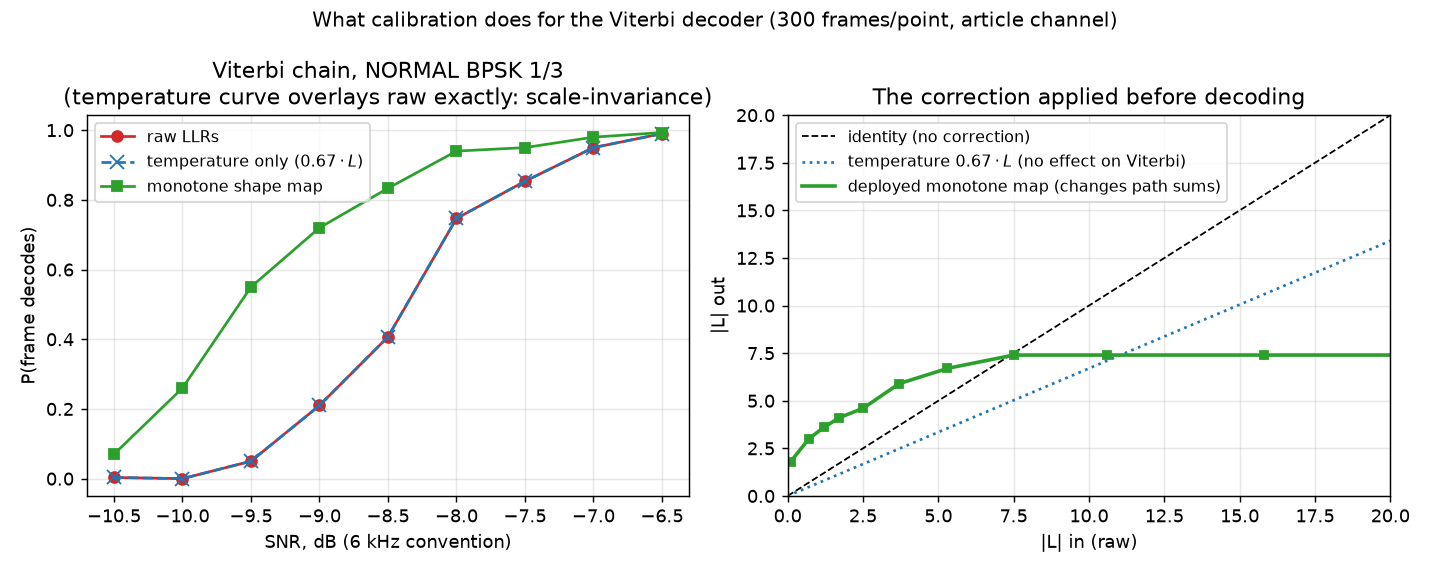
\includegraphics[width=\textwidth]{images/viterbi_recal.png}
    \caption{Calibration and the Viterbi decoder (reproduce with
             \texttt{experiments/viterbi\_recal.py}; parameters and
             per-point counts in
             \texttt{results/viterbi\_recal.json}).  Left: decode
             probability versus SNR for the same received frames
             decoded from raw LLRs, temperature-scaled LLRs
             ($0.67 \cdot L$ --- overlays raw exactly), and
             shape-mapped LLRs.  Right: the deployed monotone map
             against the identity and the temperature line: it boosts
             weak LLRs above identity and caps the top at the
             data-justified $\approx 7.4$.}
    \label{fig:viterbi_recal}
\end{figure}

\subsection{Deployment}

Alongside the static map, a per-frame temperature
$\alpha = 2\,\mathbb{E}[Lx]/\mathrm{Var}[Lx]$ is fitted from the 96
known bits of each decoded header (a Gaussian-consistency fit), which
keeps LLR scales consistent across frames --- a prerequisite for the
HARQ combining of Section~\ref{sec:coding}.  Following the
faithful-defaults principle, recalibration is \textbf{off} in the plain
\texttt{Transceiver} and enabled by the link-layer station
(\texttt{llr\_recal="auto"}).  The entire rate ladder was re-measured
with recalibration enabled; Section~\ref{sec:link} carries the
resulting sensitivities (mid-ladder BPSK/QPSK rungs gained
0.7--1.4\,dB).
